% Made up for the tikra benchmark.
\usetikzlibrary{circuits.logic.IEC, calc}
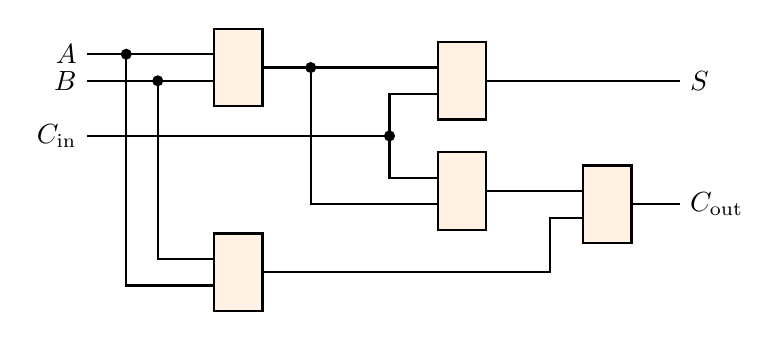
\begin{tikzpicture}[circuit logic IEC, thick, every circuit symbol/.style={fill=orange!10}]
  \node[xor gate] (x1) at (2,2) {};
  \node[xor gate, anchor=input 1] (x2) at ($(x1.output)+(2.2,0)$) {};
  \node[and gate, anchor=input 1] (a1) at ($(x1.input 1)+(0,-2.6)$) {};
  \node[and gate, anchor=input 1] (a2) at ($(x2.input 1)+(0,-1.4)$) {};
  \node[or gate, anchor=input 1] (o1) at ($(a2.output)+(1.2,0)$) {};
  \coordinate (A) at ($(x1.input 1)+(-1.6,0)$);
  \coordinate (B) at ($(x1.input 2)+(-1.6,0)$);
  \coordinate (ja) at ($(A)+(0.5,0)$);
  \coordinate (jb) at ($(B)+(0.9,0)$);
  \coordinate (jx) at ($(x1.output)+(0.6,0)$);
  \coordinate (C) at ($(B)+(0,-0.7)$);
  \coordinate (jc) at ($(C -| x2.input 2)+(-0.6,0)$);
  \draw (A) node[left] {$A$} -- (x1.input 1);
  \draw (B) node[left] {$B$} -- (x1.input 2);
  \draw (ja) |- (a1.input 2);
  \draw (jb) |- (a1.input 1);
  \draw (x1.output) -- (x2.input 1);
  \draw (C) node[left] {$C_\mathrm{in}$} -- (jc) |- (x2.input 2);
  \draw (jx) |- (a2.input 2);
  \draw (jc) |- (a2.input 1);
  \draw (a2.output) -- (o1.input 1);
  \draw (a1.output) -| ($(o1.input 2)+(-0.4,0)$) -- (o1.input 2);
  \draw (x2.output) -- ($(x2.output -| o1.output)+(0.6,0)$) node[right] {$S$};
  \draw (o1.output) -- ++(0.6,0) node[right] {$C_\mathrm{out}$};
  \foreach \j in {ja,jb,jx,jc} \fill (\j) circle (2pt);
\end{tikzpicture}
